%%%%%%%%%%%%%%%%%%%%%%%%%%%%%%%%%% DRX In situ

\subsection{Difração de raios X in situ}
\begin{frame}{Resultados}{Difração de raios X \textit{in situ}}
	\begin{itemize}
		\item Mapa representativo da condição TT170°C - TP300°C / 2h
		\item Eixo X: $2\theta$; eixo Y: Tempo de partição [s]
		\item<3-> Evolução do pico (111)$\gamma$: atenuação e deslocamento para menores valores de $2\theta$
	\end{itemize}

	\begin{figure}
		\centering
		\includegraphics<1>[width=.9\textwidth]{/home/arthur/texto_tese/img/XTMS/map_TT170TP250_waterfall.pdf}
		\includegraphics<2>[width=.9\textwidth]{/home/arthur/texto_tese/img/XTMS/map_TT170TP250.pdf}
		\includegraphics<3>[width=.9\textwidth]{/home/arthur/texto_tese/img/XTMS/map_TT170TP250_2.pdf}
	\end{figure}
\end{frame}

\begin{frame}{Resultados}{Difração de raios X \textit{in situ}}
	\begin{itemize}
		\item TT novamente fixa em 170 °C
		\item Fração do produto isotérmico $\alpha\text{-iso}$ é sempre crescente
		\item<2> Apenas na condição de partição a 450 °C toda austenita é consumida
	\end{itemize}

	\begin{figure}
		\centering
		\includegraphics<1>[width=.9\textwidth]{/home/arthur/texto_tese/img/XTMS/f_alpha-iso_QP.eps}
		\includegraphics<2>[width=.9\textwidth]{/home/arthur/texto_tese/img/XTMS/f_gamma_QP.eps}
	\end{figure}
\end{frame}

\begin{frame}{Resultados}{Difração de raios X \textit{in situ}}
	\begin{itemize}
		\item Em todas condições $\gamma$ enriquece em carbono (até 0,8\%)
		\item TP = 250 °C: menor enriquecimento em carbono, embora $f_{\alpha\text{-iso}}$ semelhante a TP = 300 e 375 °C $\rightarrow$ ferrita bainítica com maior teor de carbono ou precipitação de carbonetos.
	\end{itemize}

	\begin{figure}
		\centering
		\includegraphics<1>[width=.9\textwidth]{/home/arthur/texto_tese/img/XTMS/DwC_QP.eps}
		\includegraphics<2>[width=.8\textwidth]{img/modelos/Fe-C_meta.pdf}
	\end{figure}
\end{frame}

\begin{frame}{Resultados}{Difração de raios X \textit{in situ}}
	\begin{itemize}
		\item Curvas de transformação e enriquecimento em carbono aprentam mesmas tendências (mesmas taxas)
		\item Fortemente sugere que reação bainítica é o principal mecanismo de redistribuição de carbono
	\end{itemize}
\end{frame}
%\begin{frame}[t]{Resultados}{Difração de raios X \textit{in situ}}
	%\begin{block}{Carbono dissolvido em $\alpha$}
		%\begin{itemize}
			%\item $\%w_C^0$ estimado pelo Thermo-Calc\textregistered{} em 0,76\%
			%\item $\%w_C^\alpha \cdot f^\alpha + \%w_C^\gamma \cdot f^\gamma = \%w_C^0$\\
					%$f^\alpha + f^\gamma = 1$
		%\end{itemize}
%
		%\begin{columns}[T]
		%\begin{column}{6cm}
			%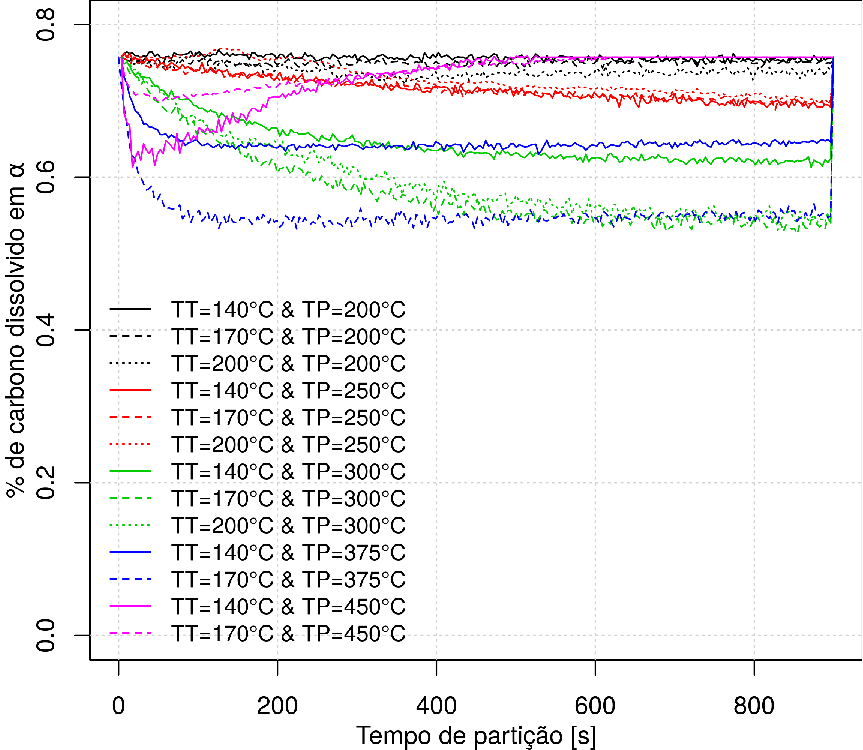
\includegraphics[width=6cm]{img/XTMS/wC_alpha.pdf}
		%\end{column}
%
		%\begin{column}{4cm}
			%\begin{itemize}
				%\item Teor de carbono dissolvido em $\alpha$ nunca inferior a 0,5\%
				%\item Supersaturação não é eliminada ou ocorre ppt. de terceira fase
				%\item No entanto, evidência de ppt. de carbonetos é conclusiva apenas a TP=450 °C
			%\end{itemize}
		%\end{column}
		%\end{columns}
	%\end{block}
%\end{frame}

%\begin{frame}[t]{Resultados}{Difração de raios X \textit{in situ}}
	%\begin{block}{Comparação com modelo ERC e valores experimentais de $f^\gamma$}
	%\begin{itemize}
		%\item Valores experimentais consistentemente inferiores a valores previstos pelo modelo ERC de Speer
		%\item Isso é justificado pela supersaturação da martensita/precipitação de carbonetos e pela própria reação bainítica, que começa antes de que a redistribuição %de carbono entre $\alpha\text{\textquoteright}$ e $\gamma$ aconteça
	%\end{itemize}
%
	%\includegraphics[width=6cm]{img/ERCxEXP.pdf}
	%\end{block}
%\end{frame}